\documentclass[a4paper, 12pt, french]{article}
\usepackage[utf8]{inputenc}
\usepackage[T1]{fontenc}
\usepackage{babel}

%Images
\usepackage{graphicx} 
\graphicspath{{src/dev/}}

%Code
\usepackage{listings}
\usepackage{color}

\definecolor{dkgreen}{rgb}{0,0.6,0}
\definecolor{gray}{rgb}{0.5,0.5,0.5}
\definecolor{mauve}{rgb}{0.58,0,0.82}

\lstset{frame=tb,
  language=Java,
  aboveskip=5mm,
  belowskip=5mm,
  framesep=3mm,
  showstringspaces=false,
  columns=flexible,
  basicstyle={\small\ttfamily},
  numbers=none,
  numberstyle=\tiny\color{gray},
  keywordstyle=\color{blue},
  commentstyle=\color{dkgreen},
  stringstyle=\color{mauve},
  breaklines=true,
  breakatwhitespace=true,
  tabsize=3
}

%Commandes perso
\newcommand{\hr}{\noindent\rule{13.7cm}{0.4pt}}

%Metas
\title{Java OO}
\author{Elanis - https://github.com/Elanis/LaTeX-cheatsheets}

\begin{document}
	\maketitle

	\section{Programme par defaut}

	\begin{lstlisting}
	public class Hello {
		public static void main(String[] args) {
			System.out.println("Hello World !!!");
		}
	}
	\end{lstlisting}

	\section{Programmation orientée objet}
	\subsection{Bases}

	\begin{lstlisting}
	public class Hello {
		private int x;

		// Constructeur
		public Hello(int x) {
			this.x = x;
		}

		// Encapsulation: getter/setter
		public int getX() { return x; }
		public void setX(x) { this.x = x; }
	}
	\end{lstlisting}

	Portées disponibles:
	\begin{description}
		\item[Privé:] Mot clé \emph{private}, inaccessible hors de l'objet
		\item[Protégé:] Mot clé \emph{protected}, inaccessible hors de la hiérarchie des classes
		\item[Friendly:] \emph{Aucun mot clé}, inaccessible en dehors du package.
		\item[Public:] Mot clé \emph{public}, totalement accessible
	\end{description}

	\begin{lstlisting}
	public class Hello {
		private int x;

		// Constructeur par recopie
		public Hello(hellOther) {
			this.x = hellOther.x;
		}
	}
	\end{lstlisting}

	\begin{lstlisting}
	public class Personne {
		// Attribut statique (dependant de la classe et non de l'objet)
		private static int NB_TOTAL = 0;

		private int id;

		public Hello() {
			this.id = ++NB_TOTAL;
		}

		// Methode statique
		public static int getNbPersonne() {
			return NB_TOTAL;
		}
	}
	\end{lstlisting}

	\subsection{Heritage}

	Une classe ne peut heriter que d'une et une seule autre classe, via le mot clé \emph{extends}.

	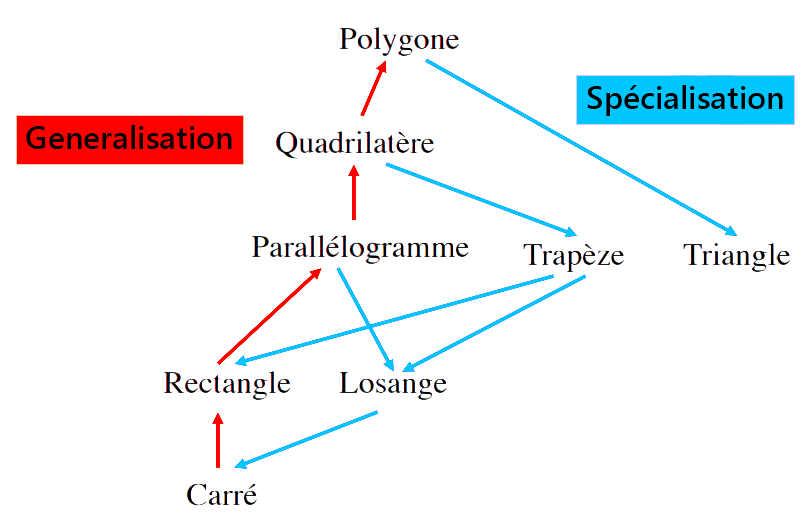
\includegraphics[width=13.8cm]{java_00_heritage}

	\begin{lstlisting}
	public class Parent {
		// ...

		public final int variable; // final = ne peut pas etre redefini dans les enfants
	}

	public class Enfant extends Parent {
		// ...
		public Enfant() {
			super(); // appelle la meme fonction du parent (ici le constructeur)
		}
	}

	public class Descendant extends Enfant {
		// ...
	}
	\end{lstlisting}

	\emph{Note:} Toutes les classes heritent implicitement de Object (java.lang.Object).\\

	\subsection{Surcharge}

	Methode \emph{toString}: appelée à chaque cast de l'objet en String. Par default il donne une representation simple de l'objet, mais on peut la surcharger comme n'importe quelle methode d'un parent.

	\begin{lstlisting}
	public class MyObject {
		// ...
		@Override
		public String toString() {
			return "Mon objet s'appelle: " + this.name;
		}
	}
	\end{lstlisting}

	\subsection{Final}

	Le mot clé \emph{final} empêche la surcharge d'une methode, la spécialisation d'une classe ou la modification d'un attribut/argument de fonction.\\

	\emph{Note:} Si un attribut final n'est pas initialisé dans sa déclaration, il devra obligatoirement être initialisé dans le constructeur.

	\begin{lstlisting}
	public class MyObject {
		final int i = 0;
		final int j;

		MyObject() {
			j = 1;
		}

		final int myFunction() {
			// ...
		}

		// ...
	}

	public class Child extends MyObject {
		// ...
		// Il est impossible ici d'ecraser i,j ou myFunction
	}

	public class A {
		// ...
	}

	public final class B extends A { // Ok
		// ...
	}

	public class C extends B { // Erreur: Impossible d'heriter d'un final
		// ...
	}
	\end{lstlisting}

	\section{Polymorphisme}

	\subsection{Classes et Methodes Abstraites}

	Une classe abstraite est une classe non instanciable, elle possede au moins une methode abstraite dont la signature est définie à l'avance mais pas le contenu.

	\begin{lstlisting}
	abstract class Shape {
		protected Point origin;

		public abstract double perimeter();
		public abstract void draw();

		@Override
		public String toString() {
			return this.getClass().getSimpleName() + " de perimetre " + this.perimeter();
			// this.getClass().getSimpleName() permet de recuperer le type de la classe instanciee.
		}
	}

	class Circle extends Shape {
		// ...
		public abstract double perimeter() {
			return 2 * Math.PI * r;
		}
		public abstract void draw() {
			// ...
		}
	}

	class Rectangle extends Shape {
		// ...
		public abstract double perimeter() {
			return 2 * (height + width);
		}
		public abstract void draw() {
			// ...
		}
	}

	Shape[] shapes = { new Circle(5), new Rectangle(3,4), new Carre(4), new Circle(3) };
	// ...
	\end{lstlisting}

	\subsection{Interfaces}

	Une interface est une classe où toutes, les methodes sont abstraites. Les methodes et lest attributes peuvent tout de même être \emph{static} ou \emph{final}. Une classe peut implementer plusieurs interfaces contrairement à l'heritage. Il faut utiliser le mot clé \emph{implements} afin d'implementer une interface.

	\begin{lstlisting}
	interface Colored {
		public void setColor(Color color);
		public Color getColor();
	}

	class Circle extends Shape implements Colored, Serializable {
		private int red, green, blue, alpha;
		// ...

		public void setColor(Color color) {
			// ...
		}
		public Color getColor() {
			return new Color(red, green, blue, alpha);
		}
	}

	class Car implements Colored {
		private Color color;
		// ...
		public void setColor(Color color) {
			// ...
		}
		public Color getColor() {
			retuen this.color.clone();
		}
	}

	Colored[] colored = { new Circle(2), new Circle(5), new Car(), new Circle(4) };
	// ...
	\end{lstlisting}

	\section{Stockage d'objets}

	\subsection{Tableaux}

	\begin{lstlisting}
	// Array (1)
	Integer[] a = new Integer(3);
	a[0] = new Integer(10);
	a[1] = new Integer(20);
	a[2] = new Integer(30);

	// Array (2)
	Integer[] b = {
		new Integer(10),
		new Integer(20),
		new Integer(30),
	};

	// For (1)
	for(int i=0; i<a.length; i++) {	
		System.out.println(a[i]);
	}

	// For (2)
	for(Integer v : a) {
		System.out.println(v);
	}
	\end{lstlisting}

	\subsection{Collections}

	Le but d'une collection est de stocker des Objet (donc tout sauf les types primitifs), d'un type, d'une classe mère, d'une implementation commune. Les collections sont plus évoluées que les tableaux, permettent de gérer des ensembles de taille dynamique.\\

	Les collections implémentent l'interface \emph{java.util.Collection}. Les 3 principales sous-interfaces sont: \emph{List<E>}, \emph{Set<E>}, \emph{SortedSet<E>}.

	\subsubsection{Vector<E>}

	\begin{lstlisting}
	Vector<String> colors = new Vector<>();

	colors.add("red");
	colors.add("green");
	colors.add("blue");

	colors.insertElementAt("yellow", 1);

	for(String c : colors) {
		System.out.println(c);
	}
	// Affichera dans l'ordre: red yellow green blue
	\end{lstlisting}

	\subsubsection{HashSet<E>}

	\begin{lstlisting}
	HashSet<String> colors = new HashSet<>();

	colors.add("red");
	colors.add("yellow");
	colors.add("green");
	colors.add("blue");

	for(String c : colors) {
		System.out.println(c);
	}
	// Affichera dans le desordre: red yellow green blue
	\end{lstlisting}

	\subsubsection{LinkedHashSet<E>}

	\begin{lstlisting}
	LinkedHashSet<String> colors = new LinkedHashSet<>();

	colors.add("red");
	colors.add("yellow");
	colors.add("green");
	colors.add("blue");

	for(String c : colors) {
		System.out.println(c);
	}
	// Affichera dans l'ordre: red yellow green blue
	\end{lstlisting}

	\subsection{Map<K,V>}

	\subsubsection{HashMap<K,V>}

	\begin{lstlisting}
	HashMap<Integer, String> personnes = new HashMap<Integer, String>();

	Integer num = 42;
	String nom = "Abc";
	personnes.put(num, nom);

	personnes.put(123456, "test");
	personnes.put(321654, "test2");

	for(Ineger cle : personnes.keySet()) {
		System.out.println(cle + " -> " + personnes.get(cle));
	}
	\end{lstlisting}

	\section{Templates Generiques}

	Le but d'un template generique est de fournir une même fonctionalité pour plusieurs types de données.

	\begin{lstlisting}
	// Par type de parametre
	public void drawAll(HashSet<? extends Shape) shapes) { // ... }
	class Groupe<P> { }

	// On peut aussi contraindre les types
	class MaClasse<P extends ClassA & InterfaceB & Autre> {
		// ...
	}
	\end{lstlisting}

	\begin{lstlisting}
	public class Personne { // ... }

	public Etudiant extends Personne { // ... }

	public class Groupe<P extends Personne> {
		ArrayList<P> groupe;

		// ...

		public void ajouter(P personne) {
			group.add(personne);
		}

		// ...
	}

	// ...

	Groupe<Etudiant> gr = new Groupe<Etudiant>();

	gr.ajouter(new Etudiant(...));
	\end{lstlisting}

	\section{Exceptions}

	\begin{lstlisting}
	try {
		// Code pouvant lever des exceptions
	} catch(Exception e) {
		// Gestion des exceptions
	} finally {
		// Sera executé ensuite, dans tout les cas
	}

	// ...

	public void myFunction(Obj param) throws NullPointerException {
		if(param == null) {
			throw new NullPointerException();
			// Peut aussi s'ecrire: throw new NullPointerException("message");
		}

		// ...
	}
	\end{lstlisting}
\end{document}